% Options for packages loaded elsewhere
\PassOptionsToPackage{unicode}{hyperref}
\PassOptionsToPackage{hyphens}{url}
\PassOptionsToPackage{dvipsnames,svgnames,x11names}{xcolor}
%
\documentclass[
  letterpaper,
  DIV=11,
  numbers=noendperiod]{scrartcl}

\usepackage{amsmath,amssymb}
\usepackage{lmodern}
\usepackage{iftex}
\ifPDFTeX
  \usepackage[T1]{fontenc}
  \usepackage[utf8]{inputenc}
  \usepackage{textcomp} % provide euro and other symbols
\else % if luatex or xetex
  \usepackage{unicode-math}
  \defaultfontfeatures{Scale=MatchLowercase}
  \defaultfontfeatures[\rmfamily]{Ligatures=TeX,Scale=1}
\fi
% Use upquote if available, for straight quotes in verbatim environments
\IfFileExists{upquote.sty}{\usepackage{upquote}}{}
\IfFileExists{microtype.sty}{% use microtype if available
  \usepackage[]{microtype}
  \UseMicrotypeSet[protrusion]{basicmath} % disable protrusion for tt fonts
}{}
\makeatletter
\@ifundefined{KOMAClassName}{% if non-KOMA class
  \IfFileExists{parskip.sty}{%
    \usepackage{parskip}
  }{% else
    \setlength{\parindent}{0pt}
    \setlength{\parskip}{6pt plus 2pt minus 1pt}}
}{% if KOMA class
  \KOMAoptions{parskip=half}}
\makeatother
\usepackage{xcolor}
\setlength{\emergencystretch}{3em} % prevent overfull lines
\setcounter{secnumdepth}{-\maxdimen} % remove section numbering
% Make \paragraph and \subparagraph free-standing
\ifx\paragraph\undefined\else
  \let\oldparagraph\paragraph
  \renewcommand{\paragraph}[1]{\oldparagraph{#1}\mbox{}}
\fi
\ifx\subparagraph\undefined\else
  \let\oldsubparagraph\subparagraph
  \renewcommand{\subparagraph}[1]{\oldsubparagraph{#1}\mbox{}}
\fi

\usepackage{color}
\usepackage{fancyvrb}
\newcommand{\VerbBar}{|}
\newcommand{\VERB}{\Verb[commandchars=\\\{\}]}
\DefineVerbatimEnvironment{Highlighting}{Verbatim}{commandchars=\\\{\}}
% Add ',fontsize=\small' for more characters per line
\usepackage{framed}
\definecolor{shadecolor}{RGB}{241,243,245}
\newenvironment{Shaded}{\begin{snugshade}}{\end{snugshade}}
\newcommand{\AlertTok}[1]{\textcolor[rgb]{0.68,0.00,0.00}{#1}}
\newcommand{\AnnotationTok}[1]{\textcolor[rgb]{0.37,0.37,0.37}{#1}}
\newcommand{\AttributeTok}[1]{\textcolor[rgb]{0.40,0.45,0.13}{#1}}
\newcommand{\BaseNTok}[1]{\textcolor[rgb]{0.68,0.00,0.00}{#1}}
\newcommand{\BuiltInTok}[1]{\textcolor[rgb]{0.00,0.23,0.31}{#1}}
\newcommand{\CharTok}[1]{\textcolor[rgb]{0.13,0.47,0.30}{#1}}
\newcommand{\CommentTok}[1]{\textcolor[rgb]{0.37,0.37,0.37}{#1}}
\newcommand{\CommentVarTok}[1]{\textcolor[rgb]{0.37,0.37,0.37}{\textit{#1}}}
\newcommand{\ConstantTok}[1]{\textcolor[rgb]{0.56,0.35,0.01}{#1}}
\newcommand{\ControlFlowTok}[1]{\textcolor[rgb]{0.00,0.23,0.31}{#1}}
\newcommand{\DataTypeTok}[1]{\textcolor[rgb]{0.68,0.00,0.00}{#1}}
\newcommand{\DecValTok}[1]{\textcolor[rgb]{0.68,0.00,0.00}{#1}}
\newcommand{\DocumentationTok}[1]{\textcolor[rgb]{0.37,0.37,0.37}{\textit{#1}}}
\newcommand{\ErrorTok}[1]{\textcolor[rgb]{0.68,0.00,0.00}{#1}}
\newcommand{\ExtensionTok}[1]{\textcolor[rgb]{0.00,0.23,0.31}{#1}}
\newcommand{\FloatTok}[1]{\textcolor[rgb]{0.68,0.00,0.00}{#1}}
\newcommand{\FunctionTok}[1]{\textcolor[rgb]{0.28,0.35,0.67}{#1}}
\newcommand{\ImportTok}[1]{\textcolor[rgb]{0.00,0.46,0.62}{#1}}
\newcommand{\InformationTok}[1]{\textcolor[rgb]{0.37,0.37,0.37}{#1}}
\newcommand{\KeywordTok}[1]{\textcolor[rgb]{0.00,0.23,0.31}{#1}}
\newcommand{\NormalTok}[1]{\textcolor[rgb]{0.00,0.23,0.31}{#1}}
\newcommand{\OperatorTok}[1]{\textcolor[rgb]{0.37,0.37,0.37}{#1}}
\newcommand{\OtherTok}[1]{\textcolor[rgb]{0.00,0.23,0.31}{#1}}
\newcommand{\PreprocessorTok}[1]{\textcolor[rgb]{0.68,0.00,0.00}{#1}}
\newcommand{\RegionMarkerTok}[1]{\textcolor[rgb]{0.00,0.23,0.31}{#1}}
\newcommand{\SpecialCharTok}[1]{\textcolor[rgb]{0.37,0.37,0.37}{#1}}
\newcommand{\SpecialStringTok}[1]{\textcolor[rgb]{0.13,0.47,0.30}{#1}}
\newcommand{\StringTok}[1]{\textcolor[rgb]{0.13,0.47,0.30}{#1}}
\newcommand{\VariableTok}[1]{\textcolor[rgb]{0.07,0.07,0.07}{#1}}
\newcommand{\VerbatimStringTok}[1]{\textcolor[rgb]{0.13,0.47,0.30}{#1}}
\newcommand{\WarningTok}[1]{\textcolor[rgb]{0.37,0.37,0.37}{\textit{#1}}}

\providecommand{\tightlist}{%
  \setlength{\itemsep}{0pt}\setlength{\parskip}{0pt}}\usepackage{longtable,booktabs,array}
\usepackage{calc} % for calculating minipage widths
% Correct order of tables after \paragraph or \subparagraph
\usepackage{etoolbox}
\makeatletter
\patchcmd\longtable{\par}{\if@noskipsec\mbox{}\fi\par}{}{}
\makeatother
% Allow footnotes in longtable head/foot
\IfFileExists{footnotehyper.sty}{\usepackage{footnotehyper}}{\usepackage{footnote}}
\makesavenoteenv{longtable}
\usepackage{graphicx}
\makeatletter
\def\maxwidth{\ifdim\Gin@nat@width>\linewidth\linewidth\else\Gin@nat@width\fi}
\def\maxheight{\ifdim\Gin@nat@height>\textheight\textheight\else\Gin@nat@height\fi}
\makeatother
% Scale images if necessary, so that they will not overflow the page
% margins by default, and it is still possible to overwrite the defaults
% using explicit options in \includegraphics[width, height, ...]{}
\setkeys{Gin}{width=\maxwidth,height=\maxheight,keepaspectratio}
% Set default figure placement to htbp
\makeatletter
\def\fps@figure{htbp}
\makeatother

\KOMAoption{captions}{tableheading}
\makeatletter
\makeatother
\makeatletter
\makeatother
\makeatletter
\@ifpackageloaded{caption}{}{\usepackage{caption}}
\AtBeginDocument{%
\ifdefined\contentsname
  \renewcommand*\contentsname{Table of contents}
\else
  \newcommand\contentsname{Table of contents}
\fi
\ifdefined\listfigurename
  \renewcommand*\listfigurename{List of Figures}
\else
  \newcommand\listfigurename{List of Figures}
\fi
\ifdefined\listtablename
  \renewcommand*\listtablename{List of Tables}
\else
  \newcommand\listtablename{List of Tables}
\fi
\ifdefined\figurename
  \renewcommand*\figurename{Figure}
\else
  \newcommand\figurename{Figure}
\fi
\ifdefined\tablename
  \renewcommand*\tablename{Table}
\else
  \newcommand\tablename{Table}
\fi
}
\@ifpackageloaded{float}{}{\usepackage{float}}
\floatstyle{ruled}
\@ifundefined{c@chapter}{\newfloat{codelisting}{h}{lop}}{\newfloat{codelisting}{h}{lop}[chapter]}
\floatname{codelisting}{Listing}
\newcommand*\listoflistings{\listof{codelisting}{List of Listings}}
\makeatother
\makeatletter
\@ifpackageloaded{caption}{}{\usepackage{caption}}
\@ifpackageloaded{subcaption}{}{\usepackage{subcaption}}
\makeatother
\makeatletter
\@ifpackageloaded{tcolorbox}{}{\usepackage[many]{tcolorbox}}
\makeatother
\makeatletter
\@ifundefined{shadecolor}{\definecolor{shadecolor}{rgb}{.97, .97, .97}}
\makeatother
\makeatletter
\makeatother
\ifLuaTeX
  \usepackage{selnolig}  % disable illegal ligatures
\fi
\IfFileExists{bookmark.sty}{\usepackage{bookmark}}{\usepackage{hyperref}}
\IfFileExists{xurl.sty}{\usepackage{xurl}}{} % add URL line breaks if available
\urlstyle{same} % disable monospaced font for URLs
\hypersetup{
  colorlinks=true,
  linkcolor={blue},
  filecolor={Maroon},
  citecolor={Blue},
  urlcolor={Blue},
  pdfcreator={LaTeX via pandoc}}

\author{}
\date{}

\begin{document}
\ifdefined\Shaded\renewenvironment{Shaded}{\begin{tcolorbox}[interior hidden, borderline west={3pt}{0pt}{shadecolor}, frame hidden, sharp corners, enhanced, boxrule=0pt, breakable]}{\end{tcolorbox}}\fi

\hypertarget{visualizing-the-2017-thomas-fire-using-landsat-imagery-and-aqi-data}{%
\subsection{Visualizing the 2017 Thomas Fire Using Landsat Imagery and
AQI
Data}\label{visualizing-the-2017-thomas-fire-using-landsat-imagery-and-aqi-data}}

Author: Zoe Zhou

\href{https://github.com/ZoeZhouJ/eds220-hwk4.git}{GitHub Repository
with Full Analysis}

\includegraphics{https://eoimages.gsfc.nasa.gov/images/imagerecords/91000/91387/ventura_er2_2017339.jpg}
Image credits: NASA

\hypertarget{about}{%
\subsubsection{About}\label{about}}

The Thomas Fire, which burned from December 2017 to January 2018, was
one of the largest wildfires in modern California history. It consumed
281,893 acres across Santa Barbara and Ventura counties, destroying
hundreds of structures and significantly impacting local ecology and
regional air quality. This blog post combines two analytical approaches:
Landsat satellite imagery for visualizing burn scars and vegetation
health, and EPA Air Quality Index (AQI) data for assessing fire-related
air quality impacts.

This case study serves multiple purposes: it demonstrates the
application of geospatial analysis techniques in environmental
monitoring, showcases the integration of multiple data sources for
comprehensive disaster assessment, and provides insights into the
environmental and public health impacts of large-scale wildfires in
California's changing climate. The analysis employs various Python-based
tools and libraries for environmental data science, making it
reproducible and adaptable for similar studies of other wildfire events.
Through this work, we aim to contribute to the growing body of knowledge
about wildfire impacts and recovery patterns in California's coastal
regions.

\hypertarget{highlights}{%
\subsubsection{Highlights}\label{highlights}}

\begin{enumerate}
\def\labelenumi{\arabic{enumi}.}
\item
  \textbf{False-Color Imaging}: Visualized vegetation health and burn
  scars using Landsat multispectral bands, revealing insights into fire
  severity and ecological recovery.
\item
  \textbf{Air Quality Assessment}: Quantified the Thomas FIre's impact
  on AQI in Santa Barbara County, using time-series data to illustrate
  pollution trends during and after the fire.
\item
  \textbf{Integrated Geospatial Analysis}: Leveraged Python libraries
  for geospatial processing, including \texttt{geopandas},
  \texttt{xarray}, and \texttt{rasterio}.
\end{enumerate}

\hypertarget{datasets}{%
\subsubsection{Datasets}\label{datasets}}

\begin{itemize}
\item
  \textbf{Landsat Surface Reflectance Data}\\
  Source:
  \href{https://planetarycomputer.microsoft.com/dataset/landsat-c2-l2}{Microsoft
  Planetary Computer - Landsat Collection 2 Level-2} This data contains
  Red, Green, Blue (RGB), Near-Infrared(NIR), and Shortwave Infrared
  (SWIR) bands. Pre-processed to remove data outside study area and
  coarsen the spatial resolution. False color image created by using the
  short-wave infrared (swir22), near-infrared, and red variables.
\item
  \textbf{Air Quality Index (AQI) Data}\\
  Source:
  \href{https://www.epa.gov/outdoor-air-quality-data}{Environmental
  Protection Agancy (EPA) - Air Data} This data contains daily AQI
  values for Santa Barbara County from 2017 to 2018.
\item
  \textbf{Thomas Fire perimeter data} Source:
  \href{https://www.fire.ca.gov/what-we-do/fire-resource-assessment-program/fire-perimeters}{CalFire}
  The database includes information on fire date, managing agency,
  cause, acres, and the geospatial boundary of the fire, among other
  information. This data was pre-processed to select only the Thomas
  fire boundary geometry.
\end{itemize}

\hypertarget{set-up}{%
\subsubsection{Set Up}\label{set-up}}

We will use the following libraries and set-up through this analysis

\begin{Shaded}
\begin{Highlighting}[]
\CommentTok{\# Import Libraries}
\ImportTok{import}\NormalTok{ pandas }\ImportTok{as}\NormalTok{ pd}
\ImportTok{import}\NormalTok{ numpy }\ImportTok{as}\NormalTok{ np}
\ImportTok{import}\NormalTok{ matplotlib.pyplot }\ImportTok{as}\NormalTok{ plt}
\ImportTok{import}\NormalTok{ os }
\ImportTok{import}\NormalTok{ geopandas }\ImportTok{as}\NormalTok{ gpd}
\ImportTok{import}\NormalTok{ rioxarray }\ImportTok{as}\NormalTok{ rioxr}
\ImportTok{import}\NormalTok{ xarray }\ImportTok{as}\NormalTok{ xr}
\ImportTok{import}\NormalTok{ matplotlib.patches }\ImportTok{as}\NormalTok{ mpatches }


\CommentTok{\# Set option to display all columns}
\NormalTok{pd.set\_option(}\StringTok{\textquotesingle{}display.max\_columns\textquotesingle{}}\NormalTok{, }\VariableTok{None}\NormalTok{)}
\end{Highlighting}
\end{Shaded}

\hypertarget{part-1-visualizing-burn-scars}{%
\subsubsection{Part 1: Visualizing Burn
Scars}\label{part-1-visualizing-burn-scars}}

\textbf{Objective}:

We will create a false-color image of the Thomas Fire to explore how
remote sensing and data visualization aid environmental monitoring.
False-color imagery, using infrared bands, highlights vegetation health,
burn severity, and fire scars. This helps assess recovery, identify
risks, and plan restoration.

\hypertarget{import-data}{%
\paragraph{Import Data}\label{import-data}}

\begin{Shaded}
\begin{Highlighting}[]
\CommentTok{\# Import landsat nc data}
\NormalTok{landsat }\OperatorTok{=}\NormalTok{ rioxr.open\_rasterio(}\StringTok{\textquotesingle{}data/landsat8{-}2018{-}01{-}26{-}sb{-}simplified.nc\textquotesingle{}}\NormalTok{)}
\CommentTok{\# Import fire boundary shapefile}
\NormalTok{thomas }\OperatorTok{=}\NormalTok{ gpd.read\_file(}\StringTok{\textquotesingle{}data/thomas{-}fire{-}boundary{-}file\textquotesingle{}}\NormalTok{)}
\end{Highlighting}
\end{Shaded}

\hypertarget{prepare-data-for-mapping}{%
\paragraph{Prepare data for mapping}\label{prepare-data-for-mapping}}

Clean redundant dimension of landsat data

\begin{Shaded}
\begin{Highlighting}[]
\CommentTok{\# Remove any length 1 dimension and its coordinates}
\NormalTok{landsat }\OperatorTok{=}\NormalTok{ landsat.squeeze().drop\_vars(}\StringTok{\textquotesingle{}band\textquotesingle{}}\NormalTok{)}
\end{Highlighting}
\end{Shaded}

After data wrangling we are ready for mapping. But first we need to
ensure coordinate reference systems (CRS) of spatial data are matched.

\begin{Shaded}
\begin{Highlighting}[]

\CommentTok{\# Match CRS for plotting}
\NormalTok{thomas }\OperatorTok{=}\NormalTok{ thomas.to\_crs(landsat.rio.crs)}

\CommentTok{\# Test for matching CRS}
\ControlFlowTok{assert}\NormalTok{ landsat.rio.crs }\OperatorTok{==}\NormalTok{ thomas.crs}
\end{Highlighting}
\end{Shaded}

Because Landsat data is downloaded with a estimated box, it's going to
be larger than the thomas fire boundary. We clip landsat with thomas
fire boundary to focus on study area.

\begin{Shaded}
\begin{Highlighting}[]
\NormalTok{thomas\_landsat }\OperatorTok{=}\NormalTok{ landsat.rio.clip\_box(}\OperatorTok{*}\NormalTok{thomas.total\_bounds)}
\end{Highlighting}
\end{Shaded}

Obtain aspect ratio with height and width to avoid distortion when
mapping

\begin{Shaded}
\begin{Highlighting}[]
\CommentTok{\# Print height and width of landsat data}
\BuiltInTok{print}\NormalTok{(}\StringTok{\textquotesingle{}Height:\textquotesingle{}}\NormalTok{, thomas\_landsat.rio.height)}
\BuiltInTok{print}\NormalTok{(}\StringTok{\textquotesingle{}Width:\textquotesingle{}}\NormalTok{, thomas\_landsat.rio.width)}

\CommentTok{\# Calculate aspect ratio for plotting }
\NormalTok{aspect\_ratio }\OperatorTok{=}\NormalTok{ thomas\_landsat.rio.width}\OperatorTok{/}\NormalTok{thomas\_landsat.rio.height}
\NormalTok{aspect\_ratio}
\end{Highlighting}
\end{Shaded}

\begin{verbatim}
Height: 149
Width: 259
\end{verbatim}

\begin{verbatim}
1.738255033557047
\end{verbatim}

\hypertarget{map-the-thomas-fire-scar}{%
\paragraph{Map the Thomas Fire Scar}\label{map-the-thomas-fire-scar}}

\begin{Shaded}
\begin{Highlighting}[]
\CommentTok{\# Initialize figure}
\NormalTok{fig, ax }\OperatorTok{=}\NormalTok{ plt.subplots(figsize }\OperatorTok{=}\NormalTok{ (}\DecValTok{8}\NormalTok{, }\DecValTok{6}\OperatorTok{*}\NormalTok{aspect\_ratio))}

\CommentTok{\# Plot landsat map by calling false image bands}
\NormalTok{(thomas\_landsat[[}\StringTok{\textquotesingle{}swir22\textquotesingle{}}\NormalTok{, }\StringTok{\textquotesingle{}nir08\textquotesingle{}}\NormalTok{, }\StringTok{\textquotesingle{}red\textquotesingle{}}\NormalTok{]]}
\NormalTok{ .to\_array()}
\NormalTok{ .plot.imshow(ax}\OperatorTok{=}\NormalTok{ax,}
\NormalTok{              robust}\OperatorTok{=}\VariableTok{True}\NormalTok{))}

\CommentTok{\# Overlay thomas fire boundary }
\NormalTok{thomas.boundary.plot(ax}\OperatorTok{=}\NormalTok{ax,}
\NormalTok{                    edgecolor}\OperatorTok{=}\StringTok{"blue"}\NormalTok{,}
\NormalTok{                    linewidth}\OperatorTok{=}\DecValTok{1}\NormalTok{,}
\NormalTok{                    label}\OperatorTok{=}\StringTok{\textquotesingle{}Thomas Fire Boundary\textquotesingle{}}\NormalTok{)}

\CommentTok{\# Add legend}
\CommentTok{\# Create a legend for the false color bands and boundary}
\NormalTok{legend\_swir }\OperatorTok{=}\NormalTok{ mpatches.Patch(color }\OperatorTok{=} \StringTok{"\#eb6a4b"}\NormalTok{, label }\OperatorTok{=} \StringTok{\textquotesingle{}Shortwave Infrared }\CharTok{\textbackslash{}n}\StringTok{ {-} Burned Area\textquotesingle{}}\NormalTok{)}
\NormalTok{legend\_nir }\OperatorTok{=}\NormalTok{ mpatches.Patch(color }\OperatorTok{=} \StringTok{"\#a1fc81"}\NormalTok{, label }\OperatorTok{=} \StringTok{\textquotesingle{}Near Infrared }\CharTok{\textbackslash{}n}\StringTok{ {-} Vegetation\textquotesingle{}}\NormalTok{)}
\NormalTok{legend\_bound }\OperatorTok{=}\NormalTok{ mpatches.Patch(color }\OperatorTok{=} \StringTok{"blue"}\NormalTok{, label }\OperatorTok{=} \StringTok{\textquotesingle{}Thomas Fire Boundary\textquotesingle{}}\NormalTok{)}
\CommentTok{\# Clean up map}
\NormalTok{ax.legend(handles }\OperatorTok{=}\NormalTok{ [legend\_swir, legend\_nir, legend\_bound], loc }\OperatorTok{=} \StringTok{\textquotesingle{}upper right\textquotesingle{}}\NormalTok{)}
\NormalTok{ax.set\_title(}\StringTok{\textquotesingle{}False Color Map with the Thomas Fire Boundary\textquotesingle{}}\NormalTok{)}
\NormalTok{plt.show()}
\end{Highlighting}
\end{Shaded}

\begin{figure}[H]

{\centering 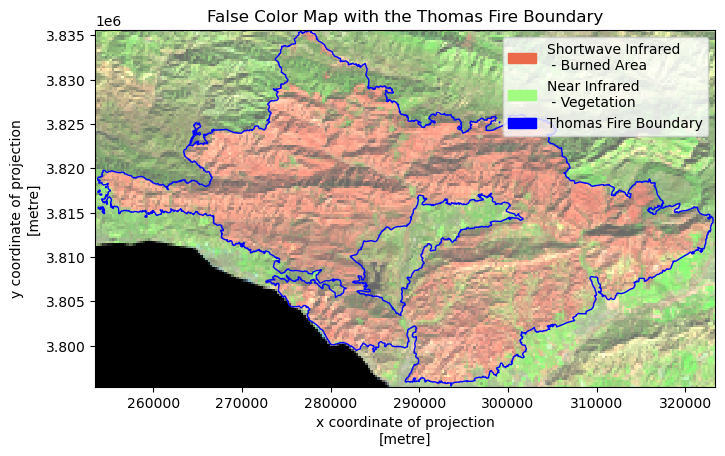
\includegraphics{spatial_analysis_thomas_fire_files/figure-pdf/cell-8-output-1.png}

}

\end{figure}

\textbf{Figure 1. False Color Map of the 2017 Thomas Fire}

This map displays the 2017 Thomas Fire region using false-color imagery
derived from Landsat data. The pinkish/salmon colored area within the
blue boundary line represents the burn scar from the Thomas Fire. The
bright green areas surrounding the burn scar represent healthy, unburned
vegetation. Using SWIR (shortwave infrared), NIR (near infrared), and
red bands is particularly effective for burn scar analysis because:

\begin{itemize}
\tightlist
\item
  SWIR is sensitive to burn scars and can penetrate smoke
\item
  NIR helps distinguish between burned and unburned vegetation
\item
  Red light helps with overall land feature distinction
\end{itemize}

This visualization enhances the identification of burn scars, vegetation
health, and moisture content.

\hypertarget{part-2-analyzing-fire-impact-on-aqi}{%
\subsubsection{Part 2: Analyzing Fire Impact on
AQI}\label{part-2-analyzing-fire-impact-on-aqi}}

\textbf{Objective}:

This part of the analysis shows the dramatic impact of the Thomas Fire
on Santa Barbara's air quality. The study built time series
visualization showing clear air quality change during fire period. A 5
day rolling averages is created to smooth daily fluctuations and
identify trends.

\hypertarget{import-data-1}{%
\paragraph{Import Data}\label{import-data-1}}

\begin{Shaded}
\begin{Highlighting}[]
\CommentTok{\# Read in data}
\NormalTok{aqi\_17 }\OperatorTok{=}\NormalTok{ pd.read\_csv(}\StringTok{\textquotesingle{}data/daily\_aqi\_by\_county\_2017.zip\textquotesingle{}}\NormalTok{, compression}\OperatorTok{=}\StringTok{\textquotesingle{}zip\textquotesingle{}}\NormalTok{)}
\NormalTok{aqi\_18 }\OperatorTok{=}\NormalTok{ pd.read\_csv(}\StringTok{\textquotesingle{}data/daily\_aqi\_by\_county\_2018.zip\textquotesingle{}}\NormalTok{, compression}\OperatorTok{=}\StringTok{\textquotesingle{}zip\textquotesingle{}}\NormalTok{)}
\end{Highlighting}
\end{Shaded}

\hypertarget{prepare-aqi-tables-for-analysis}{%
\paragraph{Prepare AQI Tables for
Analysis}\label{prepare-aqi-tables-for-analysis}}

We combined AQI data from 2017-2018 to analyze air quality trends during
the Thomas Fire period. After merging the datasets, we filtered
specifically for Santa Barbara County and removed unnecessary columns to
streamline the analysis.

\begin{Shaded}
\begin{Highlighting}[]
\CommentTok{\# concatenate tables}
\NormalTok{aqi }\OperatorTok{=}\NormalTok{ pd.concat([aqi\_17,aqi\_18])}

\CommentTok{\# Clean column names}
\NormalTok{aqi.columns }\OperatorTok{=}\NormalTok{ (aqi.columns}
\NormalTok{                  .}\BuiltInTok{str}\NormalTok{.lower()}
\NormalTok{                  .}\BuiltInTok{str}\NormalTok{.replace(}\StringTok{\textquotesingle{} \textquotesingle{}}\NormalTok{,}\StringTok{\textquotesingle{}\_\textquotesingle{}}\NormalTok{))}

\CommentTok{\# Select data from SB county and store as variable}
\NormalTok{aqi\_sb }\OperatorTok{=}\NormalTok{ aqi[aqi[}\StringTok{\textquotesingle{}county\_name\textquotesingle{}}\NormalTok{] }\OperatorTok{==} \StringTok{\textquotesingle{}Santa Barbara\textquotesingle{}}\NormalTok{] }

\CommentTok{\# Drop unnecessary columns in SB}
\NormalTok{aqi\_sb }\OperatorTok{=}\NormalTok{ aqi\_sb.drop(columns}\OperatorTok{=}\NormalTok{[}\StringTok{\textquotesingle{}state\_name\textquotesingle{}}\NormalTok{,}\StringTok{\textquotesingle{}county\_name\textquotesingle{}}\NormalTok{,}\StringTok{\textquotesingle{}state\_code\textquotesingle{}}\NormalTok{,}\StringTok{\textquotesingle{}county\_code\textquotesingle{}}\NormalTok{])}

\CommentTok{\# Verify operations }
\NormalTok{aqi\_sb.head(}\DecValTok{3}\NormalTok{)}
\end{Highlighting}
\end{Shaded}

\begin{longtable}[]{@{}lllllll@{}}
\toprule()
& date & aqi & category & defining\_parameter & defining\_site &
number\_of\_sites\_reporting \\
\midrule()
\endhead
28648 & 2017-01-01 & 39 & Good & Ozone & 06-083-4003 & 12 \\
28649 & 2017-01-02 & 39 & Good & PM2.5 & 06-083-2011 & 11 \\
28650 & 2017-01-03 & 71 & Moderate & PM10 & 06-083-4003 & 12 \\
\bottomrule()
\end{longtable}

\hypertarget{time-series-processing}{%
\paragraph{Time Series Processing}\label{time-series-processing}}

To address daily fluctuations and provide a clearer trend, we will
implement a 5-day rolling average. This method smooths the data by
averaging values over a sliding 5-day window, ensuring that short-term
variations are minimized while preserving the overall pattern in the
dataset.

\begin{Shaded}
\begin{Highlighting}[]
\CommentTok{\# Convert dates to datetime date type}
\NormalTok{aqi\_sb.date }\OperatorTok{=}\NormalTok{ pd.to\_datetime(aqi\_sb.date)}
                     
\CommentTok{\# Assign date column as index}
\NormalTok{aqi\_sb }\OperatorTok{=}\NormalTok{ aqi\_sb.set\_index(}\StringTok{\textquotesingle{}date\textquotesingle{}}\NormalTok{)}

\CommentTok{\# Define a new column in aqi\_sb}
\NormalTok{aqi\_sb[}\StringTok{\textquotesingle{}five\_day\_average\textquotesingle{}}\NormalTok{] }\OperatorTok{=}\NormalTok{ aqi\_sb[}\StringTok{\textquotesingle{}aqi\textquotesingle{}}\NormalTok{].rolling(}\StringTok{\textquotesingle{}5D\textquotesingle{}}\NormalTok{).mean()}
\end{Highlighting}
\end{Shaded}

\hypertarget{visualization}{%
\paragraph{Visualization}\label{visualization}}

We can create a visualization that displays daily AQI values alongside
the smoothed 5-day rolling average, using \texttt{matplotlib}. This plot
provides a clear view of short-term fluctuations and overall trends.

\begin{Shaded}
\begin{Highlighting}[]
\CommentTok{\# Create a plot}

\NormalTok{ax }\OperatorTok{=}\NormalTok{ (aqi\_sb.drop(columns}\OperatorTok{=}\StringTok{\textquotesingle{}number\_of\_sites\_reporting\textquotesingle{}}\NormalTok{) }\CommentTok{\# Drop unnecessary column}
\NormalTok{        .plot(title}\OperatorTok{=}\StringTok{\textquotesingle{}Daily AQI and 5{-}day average AQI in Santa Barbara from 2017 to 2018\textquotesingle{}}\NormalTok{,}
\NormalTok{              ylabel}\OperatorTok{=}\StringTok{\textquotesingle{}Air Quality Index\textquotesingle{}}\NormalTok{,}
\NormalTok{              color}\OperatorTok{=}\NormalTok{[}\StringTok{\textquotesingle{}salmon\textquotesingle{}}\NormalTok{,}\StringTok{\textquotesingle{}blue\textquotesingle{}}\NormalTok{] }
\NormalTok{)}
\NormalTok{)                                     }
\CommentTok{\# Show the date of the Thomas fire}
\NormalTok{plt.axvline(x }\OperatorTok{=} \StringTok{\textquotesingle{}2017{-}12{-}04\textquotesingle{}}\NormalTok{, }
\NormalTok{            color }\OperatorTok{=} \StringTok{\textquotesingle{}red\textquotesingle{}}\NormalTok{, }
\NormalTok{            linestyle }\OperatorTok{=} \StringTok{\textquotesingle{}dashed\textquotesingle{}}\NormalTok{, }
\NormalTok{            label }\OperatorTok{=} \StringTok{"Thomas Fire"}\NormalTok{)   }
\NormalTok{plt.legend()                  }
\end{Highlighting}
\end{Shaded}

\begin{verbatim}
<matplotlib.legend.Legend at 0x7ff0dedbd890>
\end{verbatim}

\begin{figure}[H]

{\centering 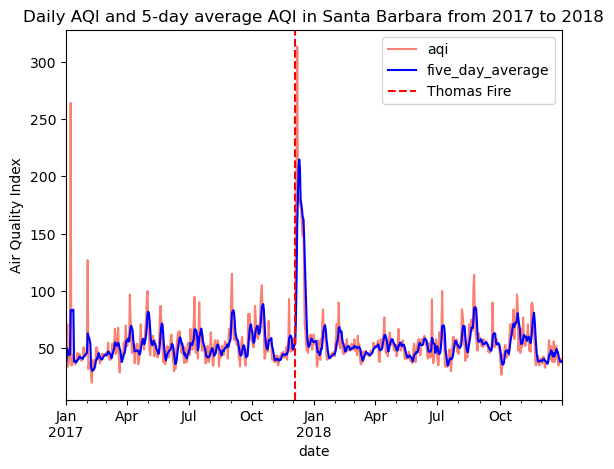
\includegraphics{spatial_analysis_thomas_fire_files/figure-pdf/cell-12-output-2.png}

}

\end{figure}

\textbf{Figure 2. Daily AQI and 5-day AQI averages in Santa Barbara
County}

During the peak fire period in December 2017, AQI values spiked
significantly above normal levels. The 5-day rolling average helps
smooth out daily fluctuations while still highlighting the severe
deterioration in air quality during the fire. Outside of the fire
period, Santa Barbara generally maintained good air quality with AQI
values typically below 100. This makes the fire's impact even more
striking, as 5-day AQI values rose well above 200 during the incident.



\end{document}
